\documentclass[paper=a4, fontsize=10pt, oneside]{scrartcl}
\usepackage[utf8x]{inputenc}
\usepackage[parfill]{parskip}
\usepackage[center]{caption}
\usepackage{graphicx}
\usepackage{sectsty}
\allsectionsfont{\centering \normalfont\scshape}
\usepackage{listings}
\usepackage{changepage}

\title{NLP homework2}
\author{Richa Jean Pierre }
\date{May 2019}


\begin{document}


\maketitle

\begin{adjustwidth}{-60pt}{-60pt}
\section{Project description}

Sense embeddings is a new way for representing a document's vocabulary.
Like word embeddings in Word2Vec, where each word in a vocabulary is represented by a vector that is learned and updated through seeing the same word in different contexts, sense embeddings are the same, but they were created to solve the problem of the ambiguity of the words. Each word can have different meanings, depending on the context it appears into, so in sense embeddings, instead of having one vector representing each word, we end up having a vector for each sense, where the sense represents a concept depending on the context it appears into.

In this project, we had a dataset in xml files containing texts and annotations for key words that appear in the text, where each annotation contained the anchor, lemma, babelnet synset(set of synonyms) each represented by the babelnet tag(bn) and a number representing the concept behind the word in this specific context, and other useful details about each word.

Our goal is to learn the embeddings that best represent the senses and test the score of a set of words similarities with respect to the scores of a human annotated gold dataset (\textbf{wordsim353}), in order to calculate the correlation between the 2 sets.

\section{Implementation}

First of all, I parsed the xml file into a json dictionary containing the text and annotations, where the annotations included the anchor(representing the word(same as it is appearing in the text), the lemma(the base of the word) and the babelNet synset(bn:number (representing the sense)). After that I replaced the words in the text by the concatenated lemma, underscore and synset (lemma\_synset), taking into account the composed words (e.g., words containing "-"), relative to each word, then I saved all the texts into a list of lists, where each list containing the final text(sentence) containing the lemma\_synset tags, instead of the original words.

After having the list of lists of sentences, it can be fed to the network to learn the embeddings. For the learning phase, I used the Gensim implementation of Word2Vec CBOW. Gensim takes parameters, from which I will be talking about the most important ones, which are the ones that I tuned during the training in order to find the best hyperparameters that fit our problem.

Different sets of hyperparameters such as (min\_count, window, embedding size, sample, learning rate, negative sampling, epochs) were tested during the training taking in the end the best combination.

After training the model, I read the gold dataset folder, which contained a human scored set of pairs of words depending on the similarity between each pair. I put the scores of pairs of words (e.g.,([love, sex]))from the gold dataset in a list, and took all the senses (lemma\_synset(s)) from the model output (e.g.,['love\_bn:00052121n',..] ['sex\_bn:00070772n',..]) relevant to each of the pairs of words in the gold dataset and calculated cosine similarity scores between each pair of senses and put the maximum from each pair in a list. After having the scores from the gold dataset and from the model output, I performed the spearman correlation to check the correlation between the 2 lists, to finaly know how the model is performing.

\section{Dataset, Hyperparameters Tuning and results}

The training was done using the eurosense datasets (high coverage or high precision), where the model performed better on the high coverage dataset. I also tried to use the SEW dataset, because the Eurosense dataset is highly biased and does not include a big variety of examples for all the senses, since it is based on governmental data, but my computer crashed 2 times and almost lost all my data, so I didn't use it in the end due to hardware limitations.

(Table \ref{table}) contain a portion of the training (and not all of the trials), due to space limitations in the report). The min\_count parameter for example is the minimum number of times a word should appear in the training data in order to be considered for the training. Putting this parameter to less than 5 was introducing a lot of words that didn't have enough samples to train the model on, which was resulting in a poor performing system, hence leading to a low correlation between the model's output and the gold dataset. The best window parameter was between 5 and 10, I picked 10 seeing that it performed a little bit better, because having this number introduces a larger context for the model to learn the target word. The best embeddings sizes were 200 and 400 and it makes sense to use a large embedding size given the big vocabulary size that we had. The learning rate is characterize by two parameters in gensim(alpha, min\_alpha), where the model starts with a learning rate of alpha and decays to min\_alpha in the end of the training and the best learning rate was starting with 0.03 and ending with 0.0007. I used a negative sampling of 10 and 5, because the model performed better. Testing was also done on several number of epochs, but I chose to put 20 and 30 only, because the others were performing worse. Using the hierarchical softmax as was suggested by the paper didn't give a good performing model, but this may be different if the SEW dataset was used. Finally the best accuracy that I got was 28.59\% as shown in (Table \ref{table})

\section{Future work}

Given that I couldn't use another dataset, doesn't make my model one of the best perfomrming ones, but as seen in Figure \ref{PCA}, the learned embeddings are correctly represented. As future work, I will be testing the model on another dataset, maybe using a better computer. This will for sure double the performance of the model, because the new dataset will introduce a new set of examples for each sense and more senses to the model, which will improve the correlation between the model output and the gold dataset. Using a new dataset may also need a new set of hyperparameters since I will be changing the data, but this will be further explored.
\end{adjustwidth}

\begin{figure}[b]
\hspace*{-5cm}
\centering
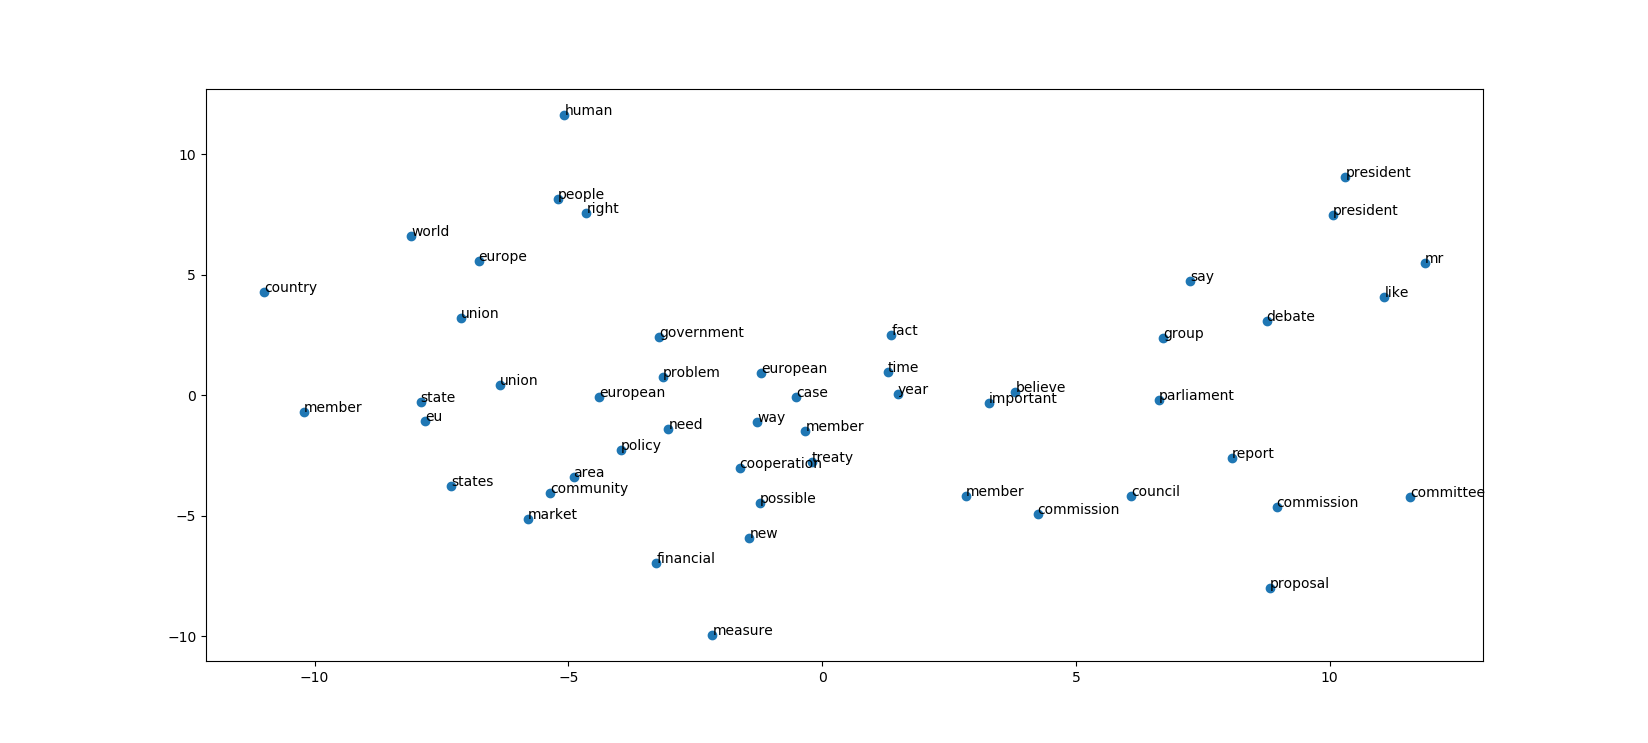
\includegraphics[width=22cm, height=14cm]{PCA.png}
\caption{Word vectors plotted using PCA for dimensionality reduction}
\label{PCA}
\end{figure}

% \textbf{\textit{Table 1}}
\begin{table}
\begin{tabular}{ |p{1.4cm}|p{1cm}|p{2.4cm}|p{2.4cm}|p{1.3cm}|p{1cm}|p{2cm}|}
 \hline
 \multicolumn{7}{|c|}{Hyperparameters} \\
 \hline
 min_count& window& embedding size& alpha:min\_alpha& negative& epochs& correlation\\

 \hline

5 &10 &200 &0.03 : 0.0007 &10 &30 &0.262890834 \\
5 &10 &400 &0.03 : 0.0007 &10 &30 &0.251853820 \\
5 &10 &200 &0.03 : 0.0007 &5 &30 &0.244147221 \\
5 &10 &400 &0.03 : 0.0007 &5 &30 &0.255396751 \\
2 &5 &200 &0.03 : 0.0007 &10 &20 &0.220916587 \\
2 &5 &400 &0.03 : 0.0007 &10 &20 &0.234543560 \\
2 &5 &200 &0.03 : 0.0007 &5 &20 &0.218193789 \\
2 &5 &400 &0.03 : 0.0007 &5 &20 &0.209779396 \\
3 &5 &200 &0.03 : 0.0007 &10 &20 &0.217164694 \\
3 &5 &400 &0.03 : 0.0007 &10 &20 &0.215683233 \\
3 &5 &200 &0.03 : 0.0007 &5 &20 &0.224217892 \\
3 &5 &400 &0.03 : 0.0007 &5 &20 &0.221486758 \\
2 &5 &200 &0.03 : 0.0007 &10 &30 &0.246600650 \\
2 &5 &400 &0.03 : 0.0007 &10 &30 &0.249965095 \\
\textbf{5} &\textbf{10} &\textbf{200} &\textbf{0.03 : 0.0007} &\textbf{10} &\textbf{30} &\textbf{0.285974860} \\
\textbf{5} &\textbf{10} &\textbf{400} &\textbf{0.03 : 0.0007} &\textbf{10} &\textbf{30} &\textbf{0.272326259} \\
5 &10 &200 &0.03 : 0.0007 &10 &20 &0.247866314 \\
5 &10 &400 &0.03 : 0.0007 &10 &20 &0.240773482 \\
5 &10 &400 &0.03 : 0.0007 &10 &30 &0.260988579 \\
5 &10 &200 &0.02 : 0.0007 &10 &20 &0.234217748 \\
5 &10 &400 &0.02 : 0.0007 &10 &20 &0.226040197 \\
5 &10 &200 &0.02 : 0.0007 &10 &30 &0.240465574 \\
5 &10 &400 &0.02 : 0.0007 &10 &30 &0.251197413 \\
5 &10 &200 &0.025 : 0.0007 &10 &20 &0.248486095 \\
5 &10 &400 &0.025 : 0.0007 &10 &20 &0.243268321 \\
5 &10 &200 &0.025 : 0.0007 &10 &30 &0.266485015 \\
5 &10 &400 &0.025 : 0.0007 &10 &30 &0.253904494 \\
2 &5 &200 &0.03 : 0.0007 &10 &30 &0.231777165 \\
2 &5 &400 &0.03 : 0.0007 &10 &30 &0.230897583 \\
2 &5 &200 &0.03 : 0.0007 &5 &30 &0.243389271 \\
2 &5 &400 &0.03 : 0.0007 &5 &30 &0.236109753 \\
2 &5 &200 &0.03 : 0.0007 &5 &30 &0.214835494 \\
 \hline
\end{tabular}
\caption{\label{table}describing the hyperparameters and their influence on the correlation accuracy between the model output and the gold dataset.}
\end{table}



\end{document}
